% !TEX root = ../main.tex
\chapter{Перший клас}


\problem
Намалюй на аркушах у~клітинку:
\begin{enumerate}
    \item трикутник, у~якого дві сторони однакові;
    \item трикутник, одна сторона якого займає 4~клітинки, а~друга~---
    2~клітинки;
    \item чотирикутник, у~якого всі сторони однакові;
    \item чотирикутник, у~якого всі сторони однакові, але не~квадрат;
    \item квадрат, який складається з~чотирьох клітинок;
    \item ще чотири квадрати, щоб кожен наступний був більший від попереднього;
    \item всередині кожного з~отриманих квадратів намалюй коло.
    Намагайся, щоб кола були якомога більшими,
    але все одно залишалися всередині квадратів.
\end{enumerate}


\problem
% TAGS: many_solutions
На нелінованому аркуші намалюй два кола (червоне та зелене)
і три цифри («один», «три», «п'ять») так,
щоб усе наступне було правдою:
\begin{itemize}
    \item цифри «один» та «п'ять» розташовані всередині червоного кола;
    \item цифри «п'ять» та «три» розташовані всередині зеленого кола;
    \item цифра «один» розташована ззовні зеленого кола.
\end{itemize}


\problem
Перед початком перерви у~Маші було шість яблук,
у~Іванки~--- чотири яблука, а~у~Федька~--- два яблука.
Це можна скорочено записати (намалювати), наприклад, так:

\medskip

\begin{tabular}{rccc}
& Маша & Іванка & Федько \\
Спочатку: & 6 & 4 & 2 \\
\end{tabular}

\medskip

Потім відбулися такі події:
\begin{enumerate}
    \item Маша дала одне яблуко Федьку;
    \item Іванка з'їла два яблука;
    \item Федько дав два яблука Іванці;
    \item Маша з'їла три яблука;
    \item Іванка віддала три яблука Федьку;
    \item Маша з'їла одне яблуко.
\end{enumerate}

Відтак перерва скінчилась і~всі пішли на наступне заняття.
Запиши (намалюй) на окремому аркуші, що відбувалося з~яблуками
та учнями протягом перерви.

Як ти думаєш:
\begin{itemize}
    \item Скільки всього було яблук на початку?
    \item Скільки всього яблук мали Іванка, Маша та Федько
    після закінчення перерви?
    \item Скільки яблук з'їли учні?
    \item Хто найменше зголоднів перед перервою? Чому?
    \item Хто найбільше зголоднів перед перервою? Чому?
\end{itemize}


\problem
Роздивися малюнок:

\begin{figure}[h]
    \centering
    
\includegraphics[width=0.8\textwidth]{1-04-1}
\end{figure}

Чи правда, що:
\begin{enumerate}
    \item всередині овалу розташовані два квадрата?
    \item ззовні кола розташовані два прямокутника?
    \item на малюнку зображено один ромб?
    \item ззовні овалу розташований квадрат?
    \item всередині овалу можна знайти три ромби?
    \item всередині фігури без кутів можна знайти прямокутник?
    \item всі фігури на малюнку різні?
\end{enumerate}



\problem
Що буде далi? Чому?
Спробуй знайти принаймнi два наступних числа (двi літери).
\begin{enumerate}
    \item 13, 15, 17, 19, \ldots
    \item 20, 17, 14, 11, \ldots
    \item 1, 1, 2, 1, 3, 1, 4, 1, \ldots
    \item 1, 1, 2, 3, 3, 5, 4, 7, \ldots
    \item 1, 2, 4, 7, 11, 16, \ldots
    \item 1, 1, 2, 3, 5, 8, 13, \ldots
    \item 1, 2, 4, 8, 16, \ldots
    \item А, В, Г, Д, Е, Ж, З, І, Ї, \ldots
    \item I, К, Н, Р, \ldots
    \item П, М, Й, И, \ldots
    \item Г, Ґ, Ж, З, Й, К, О, П, \ldots
    % в наступній послідовності літери топологічно еквівалентні
    \item Г, Ґ, И, І, Л, \ldots
\end{enumerate}


\problem
Маєш 5~шашок. Дві з них чорні, решта~--- білі.
Розташуй їх у рядочок всіма можливими способами, але так,
щоб послідовності не повторювалися.
Рішення замалюй у~зошиті.


\problem
Федько, Маша й~Іванка мешкають в~одному будинку.
Маша~--- на п’ятому поверсі, Федько~--- на 2~поверхи вище,
а~Іванка~--- одразу над Федьком.
На якому поверсі мешкає Іванка?
Скільки поверхів між помешканнями Маші й~Іванки?


\problem
% TAGS: discussion
\problemname{Теорія ймовірностей}
\begin{enumerate}
    \item В~шафці дві пари гумових чобітків різного кольору
    (або: в~мішечку 4~кубики, по 2~двох різних кольорів).
    Ти збираєшся на прогулянку і~хочеш взути пару чобітків однакового кольору,
    але дістаєш їх із~шафки наосліп. Чи пощастить?
    \item На поличці три пари рукавичок різного кольору
    (в мішечку 6~кубиків, по 2~трьох різних кольорів).
    А~тепер підбираємо однакову пару рукавичок.
    Чи вдасться піти на прогулянку в~однакових рукавичках?
\end{enumerate}


\problem
% TAGS: discussion
\problemname{Гра «Бігові доріжки»}
Є поле в~клітинку, рядки пронумеровані від~1 до~14.
Кожний розставляє свої фішки на ці «бігові доріжки».
Далі підкидають 2~гральних кубика, обчислюють суму крапочок,
які випали на гранях кубиків, і~фішка на доріжці з~таким номером
робить крок уперед.
Виграє та фішка, яка першою «добіжить» до фініша.

\emph{
Суму чисел у~грі діти рахують блискавично.
Цікаво обговорювати чому фішки, які стоять на доріжках~2, 13, 14, рухаються повільно,
а~та, що на доріжці~1~--- взагалі не може зрушити з~місця.
}


\problem
\problemname{Топологічна абетка}

\begin{figure}[h]
    \centering
    \quad \quad
    \begin{subfigure}{0.3\textwidth}
        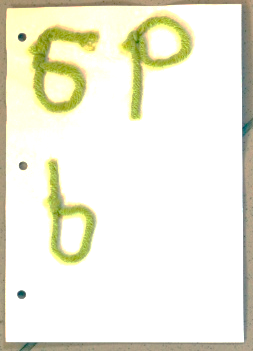
\includegraphics{1-10-1-a}
    \end{subfigure}
    \begin{subfigure}{0.3\textwidth}
        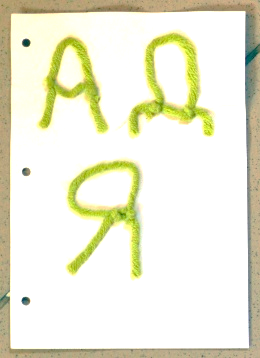
\includegraphics{1-10-2-a}
    \end{subfigure}
    \begin{subfigure}{0.3\textwidth}
        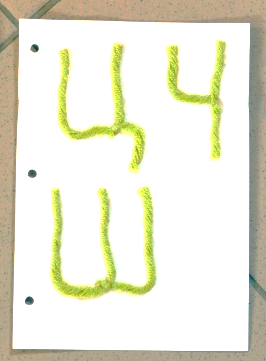
\includegraphics{1-10-3-a}
    \end{subfigure}
\end{figure}

\begin{enumerate}
    \item Знайди всі українські й англійські літери, цифри
    та математичні символи, які можна виготовити з~одного шматка мотузки.
    \item Знайди всі літери, цифри та математичні символи,
    які можна виготовити з~кільця з~одним «вусиком»;
    \item Знайди всі літери, цифри та математичні символи,
    які можна виготовити з~кільця з~двома «вусиками»;
    \item Знайди всі літери, цифри та математичні символи,
    які можна виготовити з~просто кільця («безвусого»)
    \item Знайди всі букви, цифри та математичні символи,
    які можна виготовити з~мотузочки з~язичком посередині,
    тобто вузлика з~трьома хвостиками.
\end{enumerate}

\emph{
«Заготовку» (коло з~певною кількістю вусиків) можна як завгодно вигинати,
але не можна розривати і~зв'язувати кінці.
Накладати мотузку саму на себе або клеїти вздовж,
утворюючи лінії товщиною в~дві мотузки, також не можна.
}


\problem
На правій шальці терезів 4~камінчика і~ще 5~камінчиків,
а~на лівій~--- 3~камінчика і~ще~7.
Яка шалька терезів опуститься нижче?

\emph{
Для задач на зважування у першому класі бажано використовувати
камінчики, однакові за розміром і~вагою.
Терези і~камінчики~--- не намальовані, а~справжні.
Задачу слід вирішувати на матеріальних об’єктах,
в~зошит замальовувати вже готове рішення.
}


\problem
% TAGS: many_solutions
Намалюй фігури:
\begin{enumerate}
    \item Намалюй трикутник, п'ятикутник, ромб і~коло так,
    щоб усе наступне було правдою:
    \begin{itemize}
        \item трикутник розташований всередині кола;
        \item ззовні кола немає ромба;
        \item п'ятикутник намальований навколо трикутника.
    \end{itemize}
    \item Намалюй на аркуші в~клітинку два трикутники,
    два чотирикутники і~коло так, щоб усе наступне було правдою:
    \begin{itemize}
        \item один чотирикутник рівно вдвічі більший за інший;
        \item трикутник знаходиться всередині кола;
        \item коло розташоване всередині трикутника;
        \item на малюнку немає квадратів.
    \end{itemize}
    \item Намалюй два чотирикутника, коло і~п'ятикутник так,
    щоб усе наступне було правдою:
    \begin{itemize}
        \item ромб знаходиться всередині п'ятикутника;
        \item коло розташоване навколо п'ятикутника;
        \item всередині прямокутника намальоване коло.
    \end{itemize}
    \item Напиши слово «МАТЕМАТИКА» і~намалюй два кола так,
    щоб букви «К» і~«Т» знаходилися в~різних колах,
    а~букву «М» можна було знайти всередині двох кіл одночасно.
\end{enumerate}


\problem
Завдання з терезами.
\begin{enumerate}
    \item На правій шальці терезів 10~камінчиків, а на лівій~---
    5~камінчиків і~ще~5. Яка шалька терезів опуститься нижче?
    \item З~правої шальки взяли 2~камінчики і~переклали на ліву.
    Яка шалька нижче?
\end{enumerate}
Запиши відповіді математичною мовою, застосовуючи цифри
та позначки «$=$», «$<$», «$>$».


\problem
Відтвори на терезах таку історію: $7+9 < 10+8$.


\problem
Розбий фігуру на 4~однакові частини:

\begin{figure}[h]
    \centering
    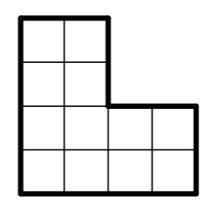
\includegraphics{1-15-1}
\end{figure}


\problem
Запиши речення математичною мовою~--- користуючись цифрами,
позначками дій («$+$» або «$-$») та знаками порівняння («$<$», «$>$», «$=$»):
\begin{enumerate}
    \item Шістнадцять і~дев'ять буде двадцять п'ять.
    \item Якщо від десяти забрати три, то вийде шість.
    \item Десять кісточок можна скласти з двох однакових купок~---
    по п'ять кісточок у~кожній.
    \item Два олівці в~лівій кишені та~ще чотири у~правій,
    разом виходить менше ніж шість олівців.
\end{enumerate}
Чи не здалося тобі щось дивним у~деяких з~цих речень?

\problem
Завдання з~терезами:
\begin{enumerate}
    \item У~ліву шальку терезів поклали чотири і~п'ять кісточок,
    а~в~праву шальку~--- три кісточки і~потім ще сім.
    Намалюй, як виглядатимуть терези.
    Одразу після цього запиши, що відбулося з~терезами,
    але математичною мовою.
    \item У~лівій шальці терезів лежить десять кісточок,
    а~у~правій~--- чотири кісточки.
    Намалюй, як виглядатимуть терези. Запиши математичною мовою.

    Коли у~праву шальку поклали камінець терези врівноважились.
    Намалюй, як виглядають терези зараз.
    Запиши математичними символами
    (замість камінця напиши знак питання «?» в~кружечку).
    Як ти думаєш, скільки кісточок важить камінець? Чому?
\end{enumerate}


\problem
Намалюй квадрат:
\begin{enumerate}
    \item кожна сторона якого проходить вздовж двох клітинок;
    \item у~два рази більший за перший;
    \item в~три рази більший за перший.
\end{enumerate}
Для кожної фігури підпиши довжини сторін.


\problem
Розкодуй слово:
\begin{enumerate}
    \item 10 11 17 1;
    \item 17 1 23 7 17 1 23 11 15 1;
    \item 27 24 15 7 21 15 1;
    \item 20 7 21 7 21 3 1.
\end{enumerate}

\emph{
Ключ до коду~--- порядковий номер літери в~абетці, тільки це таємниця.
}


\problem
Назви числа:
\begin{enumerate}
    \item по порядку за зростанням, починаючи з~випадкового числа
    в~межах $1\ldots30$;
    \item по порядку за спаданням;
    \item через одне за зростанням;
    \item через одне за спаданням.
    \item Яке третє число після 17, якщо рахувати через одне?
    \item Яке число на два випереджає 23?
\end{enumerate}


\problem
% TAGS: many_solutions
У~Марка було 6~яблук. З~них 3~були зелені, а~решта~--- червоні.
У~Іванки червоних яблук було на~2 більше, ніж у~Марка,
а~зелених~--- зовсім не було.
У~Машки було стільки~ж яблук, як і~в~Іванки.
Але були і~червоні, і~зелені. Зелених було більше.
А~у~Федька було стільки~ж зелених яблук, скільки й~у~Марка,
а~червоних~--- стільки~ж, скільки й у~Машки.
Запитання: скільки яблук було у~Федька?


\problem
% TAGS: many_solutions
Їжачок знайшов 10~яблук.
Більшу частину з~них він віддав знайомому зайцю.
Скільки яблук могло залишитись у~нього?


\problem
Запиши математичною мовою та знайди невірні (неправдиві) речення:
\begin{enumerate}
    \item Два, п'ять, сім і три~--- разом буде сімнадцять.
    \item Якщо від сімнадцяти забрати сім, то залишиться десять.
    \item Дівчинка з'їла три абрикоси вранці, а~потім чотири на обід
    і~ще дві~--- ввечері. Отже, за день вона з'їла дев'ять абрикос.
    \item В~помаранчевому мішечку лежало чотири кісточки,
    а~в~синьому~--- п'ять кісточок. Разом у~мішечках~--- дев'ять кісточок.
    \emph{Завдання з~хитринкою. В~одному випадку відповідь правдива,
    а~в~іншому~--- ні (мішечки можуть бути заховані один в~одний).}
    \item Мама купила два десятки яєць, а~потім почала робити з~них омлети.
    Щоранку вона робила омлет із~трьох яєць.
    На скільки омлетів вистачить куплених яєць? А~скільки яєць ще залишиться?
\end{enumerate}


\problem
% TAGS: many_solutions
Скільки?
\begin{enumerate}
    \item Скільки разів треба розрізати мотузочку, щоб вийшло 5~шматочків?
    Спробуй відповісти подумки, а~потім намалюй і~перевір.
    \item Скільки вузликів потрібно, щоб зв'язати 7~мотузок в~одну довгу?
    Спробуй порахувати усно, а~потім намалюй і~перевір.
    \item Скільки треба зробити розрізів, щоб перетворити кільце
    на 5~шматочків? Спробуй відповісти усно, а~потім намалюй і~перевір.
    \item Всередині синього кола три трикутника, а~всередині зеленого кола
    трикутників п'ять. Скільки всього трикутників може бути на малюнку?
    \item Хтось на мотузочці зав'язав два більших і~два менших вузлика.
    А~всього вузликів три. Спробуй здогадатися, як таке могло статися? Намалюй.
\end{enumerate}


\problem
Вгадай число:
\begin{enumerate}
    \item Я задумав число. Потім додав до нього 5. Вийшло 17.
    Яке число я задумав?
    \item Я задумав число. Потім додав до нього 5.
    Потім від того, що вийшло відняв 3. Вийшло 2.
    Яке число я задумав?
\end{enumerate}


\problem
% TAGS: discussion
Як ти вважаєш, які з~речень є правдивими? Чому?
А~які інколи бувають правдою, а~інколи неправдою? Поясни. Наведи приклади.
А~які з~речень на твою думку є неправдивими? Поясни. Виправ помилки.
\begin{enumerate}
    \item П'ять і~сім разом~--- це стільки~ж, скільки буде два рази по шість.
    \item Сімнадцять кісточок можна скласти з~трьох рядів
    по шість кісточок в~кожному.
    \item Тиждень складається з~7~днів.
    \item Місяць (той, що у календарі) складається з~30~днів.
    \item Квадрат можна назвати чотирикутником.
    \item Чотирикутник можна назвати квадратом.
\end{enumerate}


\problem
Федько зібрав поїзд з~Lego. Поїзд тягнув тепловоз, а~за ним йшли вагони.
Один лісовоз, один поштовий вагон і~декілька пасажирських вагонів.
Пасажирських вагонів у~поїзді було найбільше.
Поїзд у Федька вийшов довгий~--- 1 метр і~5~сантиметрів.
Скільки пасажирських вагонів було у~поїзді,
якщо тепловоз має довжину 25~сантиметрів, а~всі вагони~--- по 20~сантиметрів.


\problem
З~початком весни на П'ятихатках почали танути бурульки.
Женька й~Андрій кожного ранку виходили на двір і~рахували, скільки розтануло,
а~скільки залишилось.
Першого березня розтануло чотири найменших бурульки.
Другого~--- перетворились на~воду ще п'ять.
У третій день весни зникло бурульок на дві менше, ніж у~перший.
Четвертого березня розтануло стільки~ж, скільки другого.
А~п'ятого березня зранку з~даху звисало лише дві.

З'ясуй скільки бурульок було на початку.
А~скільки їх було у~кожний зі згаданих днів?
Запиши математичною мовою, як змінювалася кількість бурульок
протягом спостережень.


\problem
% TAGS: many_solutions
Слон, мишеня, заєць та папуга вирішили позмагатися, хто швидше з'їде
з~гори на лижах. Вони піднялися на вершину гори й~одночасно рушили вниз.
Дізнайся, в~якому порядку вони дісталися фінішу, якщо відомо, що:
\begin{itemize}
    \item Мишеня їхало швидше за зайця.
    \item Папуга приїхав до підніжжя гори не третім і~не першим.
    \item Слон приїхав одразу після зайця.
\end{itemize}


\problem
Валя на Масляну напекла купу млинців і~після того, як пригостила всіх
і~сама поласувала, розклала ті, що залишилися, на дві тарілки порівну.
Млинці спокійно лежали на цих двох тарілках (лівій і~правій)
аж до закінчення заняття з~математики.
Потім прибігли учні разом із Сашком і~все з'їли.
Відомо, що Федько, Марко й~Іванка їли з~правої тарілки,
а~Машка із Сашком~--- з~лівої.
Також відомо що Марко з'їв 4~млинці, Іванка~--- 3,
Машка і~Федько з'їли млинців порівну, кожний на один млинець більше за Марка.

Скільки млинців з'їв Сашко?
Спробуй стисло намалювати все що відбулося із млинцями.
Подумай, як би ти записав цю історію математичною мовою?


\problem
На ліву шальку терезів поклали 3~камінці.
Перший важить стільки, скільки й 4~кісточки.
Вага другого становить шість кісточок.
А~третього додолу тягне так само, як 2~кісточки.
На правій шальці терезів було 7~кісточок.
Але після того, як на праву шальку ще прилетів іграшковий дракон,
терези врівноважились.

Визнач, з~якою силою тягне вниз іграшкового дракона,
що сидить на правій шальці.


\problem
Федько і~Василько пішли з~татком до лісу.
Там вони гуляли поміж дерев, слухали спів пташок,
збирали жолуді й~горішки ліщини.
Василькові дуже сподобалися жолуді, тому він набрав в~кишеню більше
жолудів, ніж ліщини. А~Федько збирав ліщину, жолуді брав рідко,
тому в~його кишені було більше горішків, ніж жолудів.
Але у~Федька кишені більші, ніж у~братика, тому вмістили
більше горішків і~жолудів, ніж у~Василька.

Скільки жолудів і~горішків ліщини назбирав кожний з~братиків,
якщо вдома, коли вони висипали з~усіх кишень на стіл свої знахідки,
татко нарахував 8~жолудів і~7~горішків ліщини.


\problem
% TAGS: discussion
Які з~наступних тверджень є правдою?
\begin{enumerate}
    \item Якщо коло знаходиться всередині трикутника,
    а~трикутник знаходиться всередині квадрата,
    то коло знаходиться всередині квадрата.
    \item Якщо жовта мотузочка довша за зелену,
    а~зелена довша за червону, то жовта довша за червону.
    \item Якщо яблуко важче за камінь, а~камінь важить більше за пінопласт,
    то яблуко важче за пінопласт.
    \item Якщо равлик швидший за зайця, а~заєць швидший за страуса,
    то равлик швидший за страуса.
\end{enumerate}
Подумай, як дуже стисло записати (замалювати) кожне з~тверджень.


\problem
На заняття прийшли троє учнів: Машка, Іванка і~Федько.
І~сіли за три парти: ліву, середню і~праву.
Скількома різними способами учні можуть вибрати собі парти?
Відшукай і~схематично намалюй всі можливі варіанти.
У~скількох з~них Іванка сидить поряд із Машкою?
Скільки існує варіантів розсаджування, де Машка сидить поряд із Федьком?
Чи можна учням сісти за парти так,
щоб Машка сиділа поряд із Федьком та Іванкою одночасно?



\problem
У твоїх~руках є дві мотузочки:
одна довжиною у~5~сірників, а~друга~--- у 8~сірників.
Більше нічого в~твоїх~руках немає (сірників теж).
\begin{enumerate}
    \item Як можна відміряти шматок мотузки довжиною у~3~сірники?
    \item Як можна відміряти шматок мотузки довжиною у~4~сірники?
    \item Як можна відміряти шматок мотузки довжиною в~1~сірник?
\end{enumerate}
Запиши кожний зі знайдених способів виготовлення математичною мовою.


\problem
Чи правда, що можна намалювати коло, всередині якого знаходиться
трикутник, не відриваючи олівця від паперу?
(Крім кола та трикутника, інших ліній на малюнку не повинно бути).


\problem
Оленка живе в~будинку разом із~татом, мамою, сестрою, одним песиком,
двома котиками, двома папужками, трьома рибками та равликом.
Скільки вони всі разом мають ніг?


\problem
Було 9~аркушів паперу. Деякі з~них розрізали на три частини.
Усіх разом аркушів стало 15.
Скільки аркушів було розрізано?


\problem
Іра, Аня, Катя, Оля і~Маша мешкають в одному будинку:
двоє дівчаток на першому і~троє на другому поверхах.
Оля мешкає не на тому поверсі, що Катя і~Маша.
Аня не на тому поверсі, що Іра і~Катя.
Хто з~дівчат мешкає на першому поверсі?
